\section{Pharmacokinetics} \label{PKPD}

In this section, I introduce the central pharmacokinetic model used in this research.  I derive the model from a differential equation and examine its qualitative behavour using non-dimensionalization.  Population pharmacokinetic models are discussed as a generalization of the one compartment pharmacokinetic model


\subsection{A One Compartment Pharmacokinetic Model} 

To analyze the time course of drug mass in various parts of the body, compartmental models may be used.  These models posit that the body (or relevant organs/systems of the body) is comprised of compartments from which drug can flow in and out. The rates at which the drug can enter and exit each compartment are specified, and a differential equation for each compartment can be written down and solved using methods outlined in \cref{sec:ODE}.

An example of these models used for orally-administered drugs is the one--compartment pharmacokinetic model with first order elimination.  The model posits the following \cite{wakefield1992bayesian}:  
%
\begin{itemize}
\item The rate of drug absorption from the gut ($ G  $) into the blood plasma ($ C $) is proportional to the amount of drug in the gut and that is the proportionality constant is $ k_a $, in units $ \text{hours}^{-1} $;

\item The rate of elimination from the blood plasma is proportional to the amount of drug in the plasma compartment with proportionality constant $ k_e $, in units $ \text{hours}^{-1} $;

\item The volume of plasma in the body is $ V $, in units litres;

\item The bioavailability of the drug (i.e. the fraction of drug absorbed into the blood serum) is $F$;
\end{itemize}

The differential equation governing the mass transit if drug in/out of the $C$ compartment is then $dC(t)/dt = k_aFD\exp(-k_a t) - k_eC(t)$, and is a first order linear differential equation.  The concentration of the drug in the $C$ compartment can be obtained by dividing $C(t)$ by the volume of the $C$ compartment, $V$.  The differential equation can be non-dimensionalized by letting $\tau$ and $y(\tau)$ be the non-dimensional quantities, and letting $C(t) = k_a FD/V y(\tau)$ and $t = \tau/k_a$.  The non-dimensionalized differential equation is then

\begin{equation}
	\dfrac{dy(\tau)}{d\tau} = \exp(-\tau) - \alpha y(\tau)
\end{equation}

\noindent Here, $\alpha = k_e / k_a$ is the ratio of elimination and absorption rates, and is dimensionless.  The differential equation's qualitative behaviour depends solely on this ratio, with all parameterizations in which $\alpha$ is constant displaying the same qualitative behaviour.  The remaining variables $V$, $D$, and $F$ only serve to scale the solution vertically.  The solution to this differential equation (obtained via integrating factors or the Laplace Transform) is

\begin{equation}\label{key}
	y(\tau) = \dfrac{1}{\alpha -1} \Big( \exp(-\tau) - \exp(-\alpha \tau) \Big)
\end{equation}

\noindent which can be transformed back into dimensional variables to yield

\begin{equation}\label{onecompartment_PKPD}
	C(t) = \dfrac{F D}{V}\dfrac{k_a}{k_e - k_a}\Big(e^{-k_at} - e^{-k_et}\Big) \>.
\end{equation}

In the remainder of this thesis, \cref{onecompartment_PKPD} will be parameterized in terms of the clearance rate $Cl = V \cdot k_e$ rather than in terms of volume due to more prior information being available about the clearance rate of certain drugs as opposed to the volume of patients.  The resulting parameterization is

\begin{equation}\label{onecompartment_PKPD_cl}
	C(t) = \dfrac{F D}{Cl}\dfrac{k_ek_a}{k_e - k_a}\Big(e^{-k_at} - e^{-kt}\Big) \>.
\end{equation}

\begin{figure}[h!]
	\centering
	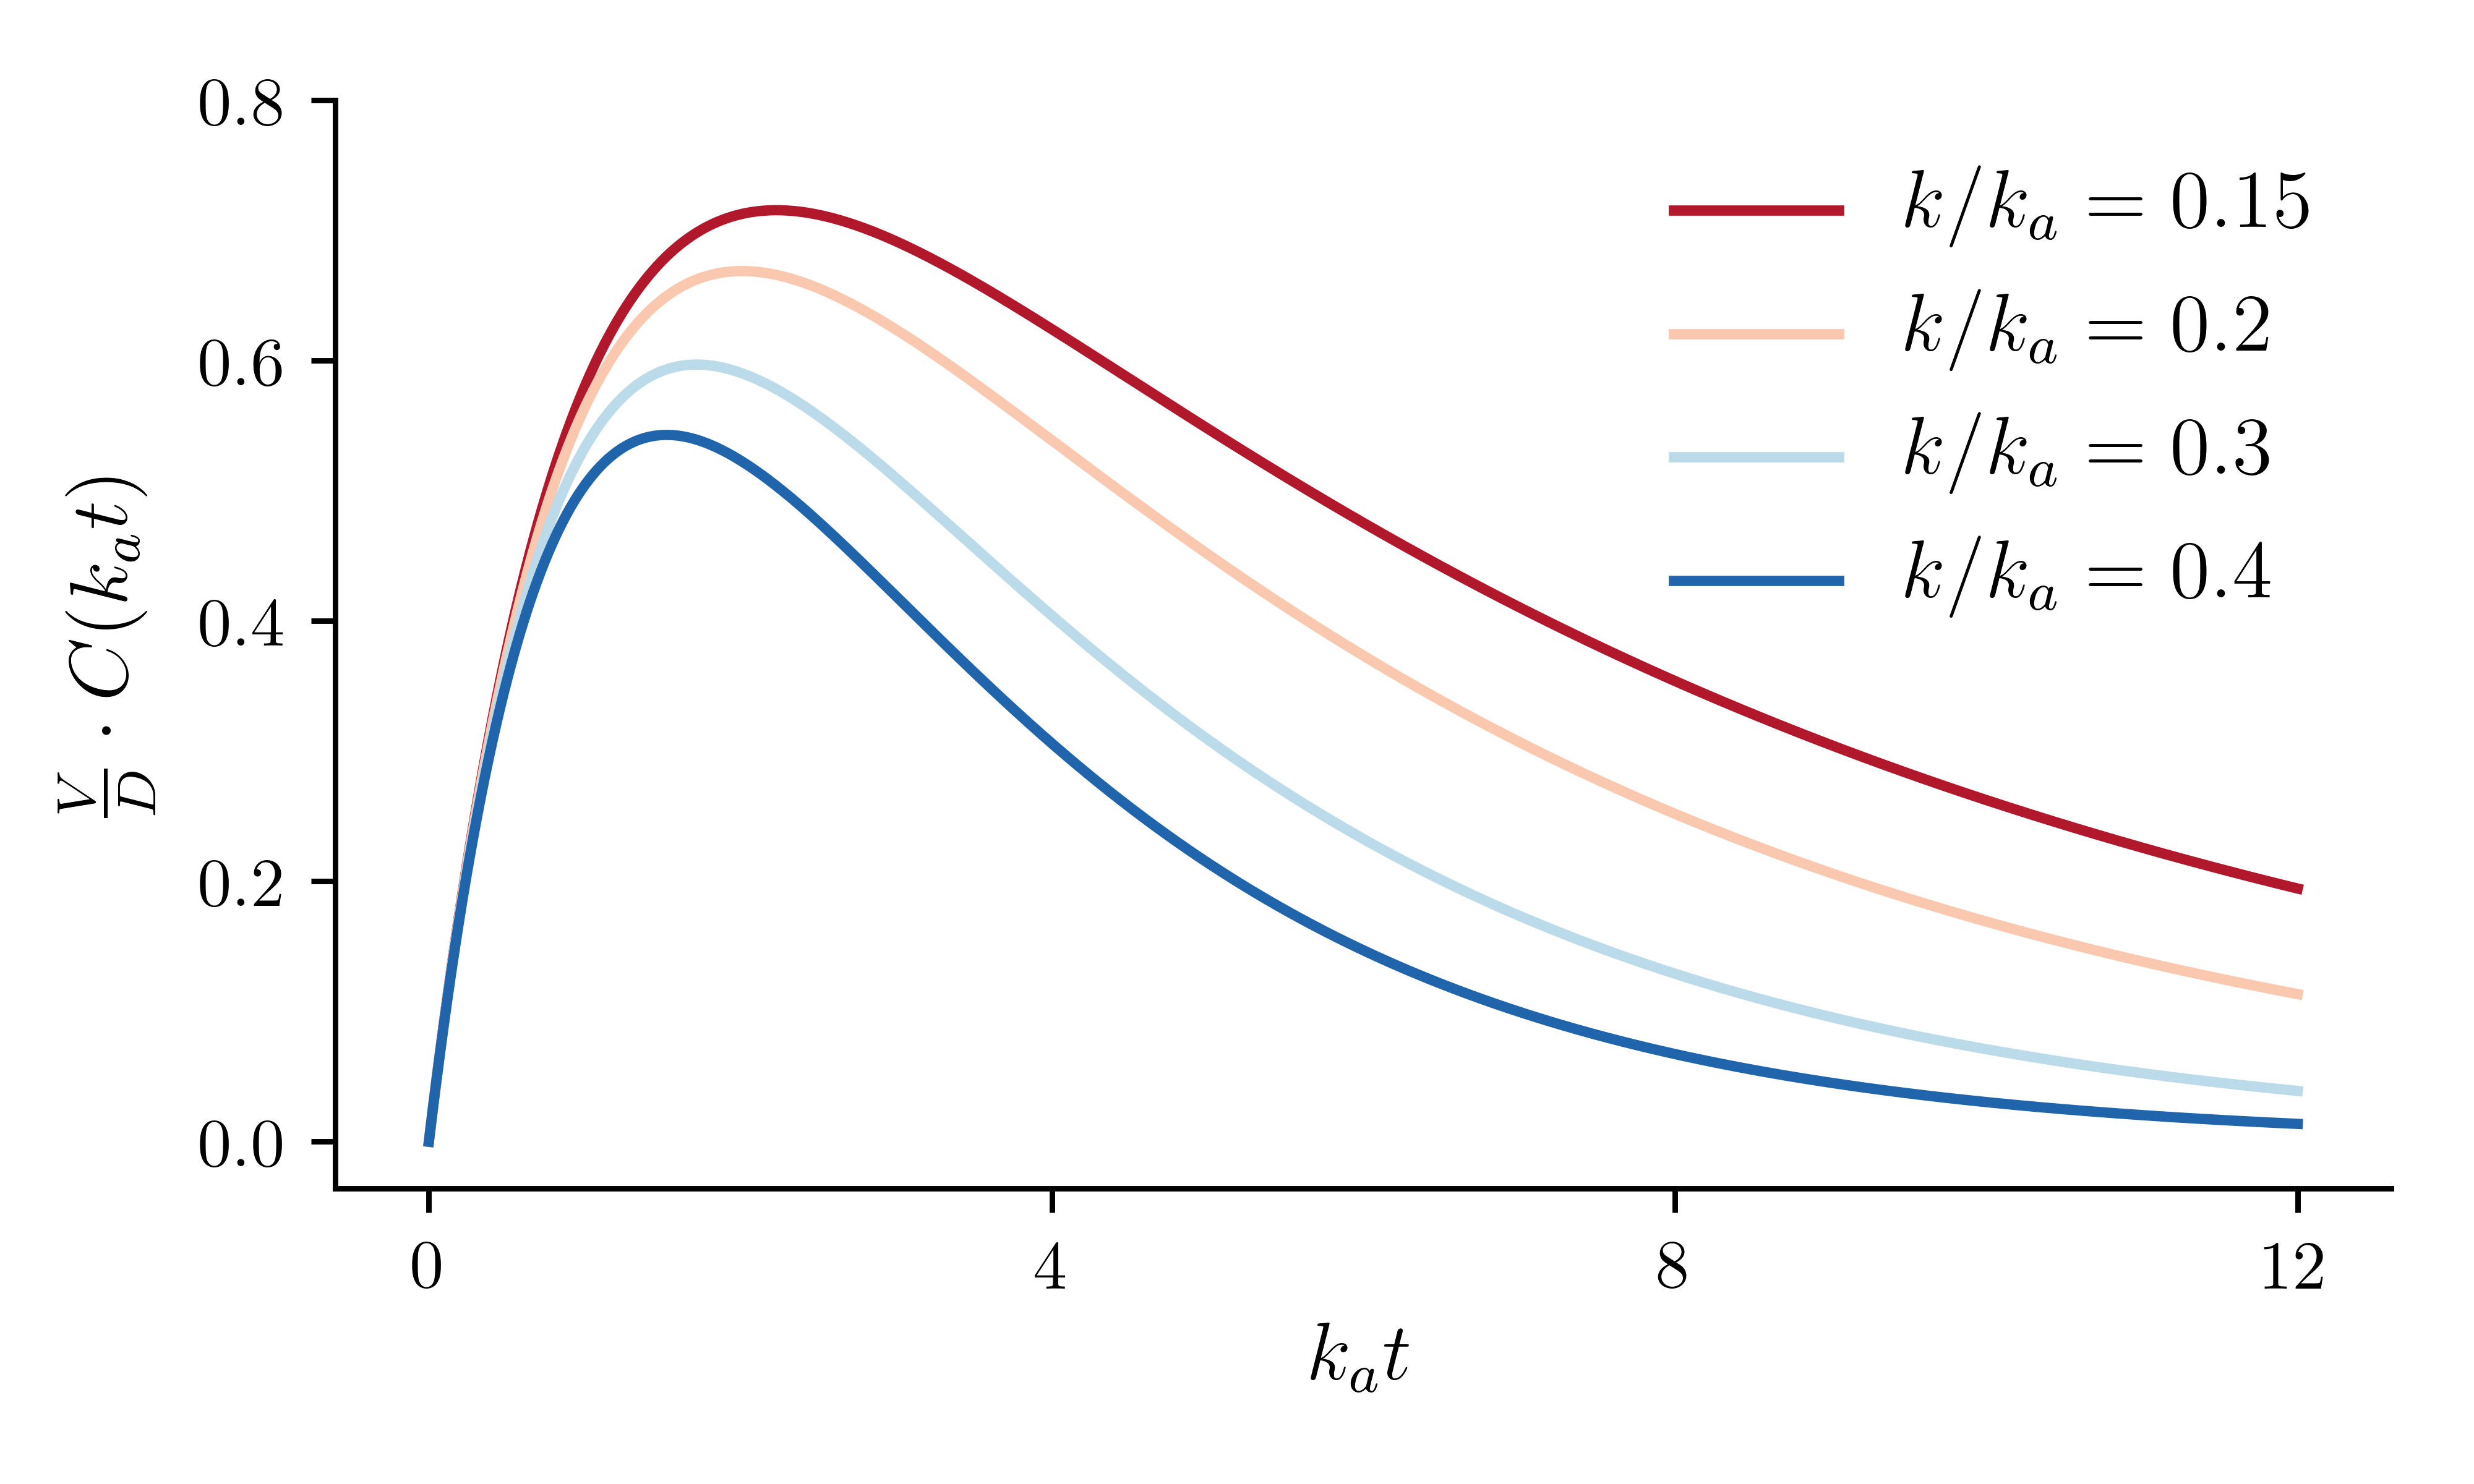
\includegraphics{figures/pkcurves.png}
	\caption[Non-dimensionalized solutions to pharmacokinetic differential equation] {Non-dimensionalized concentration plotted against non-dimensionalized time.  The process non-dimensionalizing the differential equation removes all units from the model, allowing for qualitative comparisons of the solution under different families of parameterization.  Here, it is shown that all parametrizations in which $\alpha = k_e/ka = 0.15$ elicit larger concentrations than those parameterizations in which $\alpha=0.4$ conditioned on $FD/V$ remaining constant.}
	\label{fig:pkcureves}
\end{figure}

\subsection{Population Pharmacokinetic Models}

Different patients may have different pharmacokinetics just by virtue of being different people (even if they match identically on important clinical and genetic covariates).  To understand the between subject variability in pharmacokientics, a population pharmacokinetic model can be constructed.  These models make the assumption that some or all of the parameters in \cref{onecompartment_PKPD_cl} (or some other pharmacokinetic model for that matter) are themselves random variables, which have some population level mean and variance which requires estimation.  As an example, the clearance rate for the $i^{th}$ patient in the population, $Cl_i$, can be considered as a draw from some population level distribution, $Cl_i \sim P(\mu, \sigma) $, where $P$ is some distribution with suitable support for the modelled parameter.  This approach is similar to non-linear mixed effect modelling; non-linear because the concentration function is non-linear in the pharmacokinetic parameters, and mixed-effects because the parameters are free to vary between patients \cite{mould2013basic}.

Many software packages exist to fit population pharmacokinetic models.  Notable examples  include NONMEM \cite{bauer2011nonmem} and Monolix \cite{noauthor_monolix_nodate} (both of which happen to be propriatary software) and Pumas \cite{rackauckas2020accelerated} which is freely available and accessed through the Julia language (which is also free), among others.  Each implementation shares similar techniques for parameter estimation, namely by optimizing the negative log likelihood (which is sometimes called the \textit{Objective Function} or OFV) \cite{bauer2011nonmem, mould2013basic, bauer_nonmem_2019}, as well as approximation methods for computing the marginal likelihood.  Several approximation techniques are made available to users, but the differences in resulting estimates from these methods can sometimes be substantial \cite{mould2013basic}.